\documentclass[11pt,a4paper,oneside,notitlepage]{book}
\usepackage{amsmath}                    % Uitgebreide wiskundige mogelijkheden
\usepackage{amssymb}                    % Voor speciale symbolen zoals de verzameling Z, R...
\usepackage{makeidx}                    % Om een index te maken
\usepackage{url}						% Om url's te verwerken
\usepackage{fixltx2e}
\usepackage{textcomp}            
\usepackage{graphicx}                   % Om figuren te kunnen verwerken
\usepackage{epstopdf}
\usepackage{xspace}                     % Magische spaties na een commando
\usepackage[latin1]{inputenc}           % Om niet ascii karakters rechtstreeks te kunnen typen
\usepackage{float}                      % Om nieuwe float environments aan te maken. Ook optie H!
%\usepackage{flafter}                   % Opdat floats niet zouden voorsteken
\usepackage{listings}                   % Voor het weergeven van letterlijke text en codelistings
\usepackage[round]{natbib}              % Voor auteur-jaar citaties.
\usepackage[nottoc]{tocbibind}			% Bibliografie en inhoudsopgave in ToC; zie tocbibind.dvi
\usepackage{marvosym}                   % Om het euro symbool te krijgen
%\usepackage{textcomp}                  % Voor onder andere graden celsius
%\usepackage{fancyhdr}                  % Voor fancy headers en footers.
\usepackage[small,bf,hang]{caption2}	% Voor de captions te verbeteren
\usepackage[Gray,squaren,thinqspace,thinspace]{SIunits} % Elegant eenheden zetten 
\renewcommand{\baselinestretch}{1.35}   % De interlinie afstand wat vergroten.
%\usepackage[english,dutch]{babel}
\usepackage{flafter} %nieuw
\usepackage{lscape} %nieuw
\usepackage{fancyhdr}
\usepackage{amsmath, amssymb, amsbsy}
\usepackage{verbatim} 
\usepackage{float}
\usepackage{subfigure}
\usepackage{hyperref}


% marges aanpassen
% (opmerking: moet *voor* inclusie van fancyhdr package komen)
\setlength{\hoffset}{-1in}
\setlength{\voffset}{-1in}
\setlength{\topmargin}{2cm}
\setlength{\headheight}{0.5cm}
\setlength{\headsep}{1cm}
\setlength{\oddsidemargin}{3.5cm}
\setlength{\evensidemargin}{3.5cm}
\setlength{\textwidth}{16cm}
\setlength{\textheight}{23.3cm}
\setlength{\footskip}{1.5cm}
\setlength{\parindent}{0cm}       
\setcounter{secnumdepth}{3} %nieuw


%Deftige fancy-header (hoofdstukken)
\pagestyle{fancy}
\fancyhf{}
\renewcommand{\headrulewidth}{0.5pt}
\fancyhf[HL]{\uppercase{\textit{\leftmark}}}
\fancyhf[HR]{\thepage}

\graphicspath{{images/}} % place of the figures

%\makeindex                              % Om een index te genereren.

\setcounter{MaxMatrixCols}{20}          % Max 20 kolommen in een matrix
\setcounter{tocdepth}{3}

% De headers die verschijnen bovenaan de bladzijden, herdefinieren:
\pagestyle{fancy}                       % Om aan te geven welke bladzijde stijl we gebruiken.
\fancyhf{}                              % Resetten van al de fancy settings.
\renewcommand{\headrulewidth}{0.4pt}      % Geen lijn onder de header. Zet dit op 0.4pt voor een mooie lijn.
\fancyhf[HL]{\nouppercase{\textit{\leftmark}}} % Links in de header zetten we de leftmark,
\fancyhead[HR]{\thepage}                % Rechts in de header het paginanummer.
% Activeer de volgende lijn en desactiveer de vorige om paginanummers onderaan gecentreerd te krijgen.
%\fancyhf[FC]{\thepage}                  % Paginanummers onderaan gecentreerd.

\newcommand{\npar}{\par \vspace{2.3ex plus 0.3ex minus 0.3ex}}
\newcommand{\cel}{$^{\circ}$C}


%%%%%%%%%%%%%%%%%%%%%%%%%
% Einde van de preamble.%
% Begin van de body:	  %
%%%%%%%%%%%%%%%%%%%%%%%%%

\begin{document}


\frontmatter

\title{Rover manual}
\author{Niklaas Colaert}


%  Titelblad

\begin{titlepage}

\fontsize{12pt}{14pt}\selectfont

\begin{center}

\begin{figure}[H] 
		\begin{center}
			
\includegraphics[width=3cm, height=4cm]{VIB.pdf}
			\hfill 
			
\includegraphics{ugent.pdf}
			
		\end{center}
\end{figure}



\vspace{0.3cm}


\vspace{0.8cm}
Proteomics and Bioinformatics group 
\linebreak  Departement of Medical Protein Research
\linebreak  VIB and Faculty of Medicine and Health Sciences, Ghent University
\linebreak  \url{http://www.compomics.be}


\vspace{3.2cm}

	\begin{minipage}[c][4.5cm][c]{15cm}
	\begin{center}
	\fontsize{17.28pt}{21pt}\selectfont
	{\textsc{Rover manual}}
	\fontseries{m}
	\vspace{0.2cm}
	\fontsize{12pt}{14pt}\selectfont
	\linebreak  Niklaas Colaert
	\end{center}
	\end{minipage}
	
	
\vspace{4.5cm}

\date{}
 \url{http://code.google.com/p/compomics-rover/}
\end{center}
\end{titlepage}



\tableofcontents

\mainmatter

\chapter{General Information}
\section{Downloading and running Rover}
\paragraph{}The main Rover site is \url{http://code.google.com/p/compomics-rover/}. There, under the download section, a zip file containing the program can be downloaded. The rover program can be started by double clicking the rover-2.0.jar file after unzipping the folder.
\paragraph{}The maximum number of \textit{.rov} files that can be loaded at a time is limited. The size of all the \textit{.rov} files cannot exceed the size of the virtual memory committed to Rover. Normally, the rest of the filetypes that can be loaded by Rover have smaller file sizes and the number of such files that can be loaded is thus not limited.
\paragraph{}The virtual memory that is committed to the Rover program can be changed in the rover.properties file. This file is located in the user/.compomics/rover folder. This is not the location where the program is located. The default value is 1024 Mb. This can be changed by editing the number after \textit{-Xmx} in the file.


\section{Java}
	It is probable that a functional Java is already installed on your computer due to the widespread use of Java nowadays. If you do not know for sure you have Java 1.5 or higher installed, you can do the following simple check:
	\begin{itemize}
		\item Open a command window by \texttt{start} $\rightarrow$ \texttt{run} and enter \texttt{cmd}.
		\item Enter \texttt{Java -version} in the command window.
	\end{itemize}	
	If Java is already installed, you will see something like below where x stands for the version.\begin{verbatim}{Java version "1.x.0_01"}\end{verbatim}
	If your Java version is lower then 1.5 you have to upgrade Java. If you don't have Java installed, you have to make a new install. 
	In both cases, you have to install a new Java version. The installation of Java is quite simple.
	\begin{itemize}
	\item Go to \url{http://java.com}
	\item follow the main download link and start the download
	\item when finished, open the installer and follow the straightforward instructions
\end{itemize}	


%chapter on the data input
\chapter{Starting Rover with the Rover wizard}\label{wizard}

\section{Different types of analyses}
\paragraph{}Two different types of analysis can be performed in rover. The simplest one is the analysis of quantitative data. A second methods is also available where different source of quantitative data can be combined via location and scale normalization.

\section{Starting the Rover wizard}

\paragraph{}The Rover wizard can be started by double clicking the rover.jar file in the installation directory of the Rover program. When the Rover wizard is opened correctly, a welcome screen (see figure \ref{welcome}) appears. When the multiple sources approach button 
\includegraphics[scale=0.6, H]{mutliRover.png} is clicked a different welcome screen (see figure \ref{welcome_M}) appears. 

\begin{figure}[H]
\begin{center}
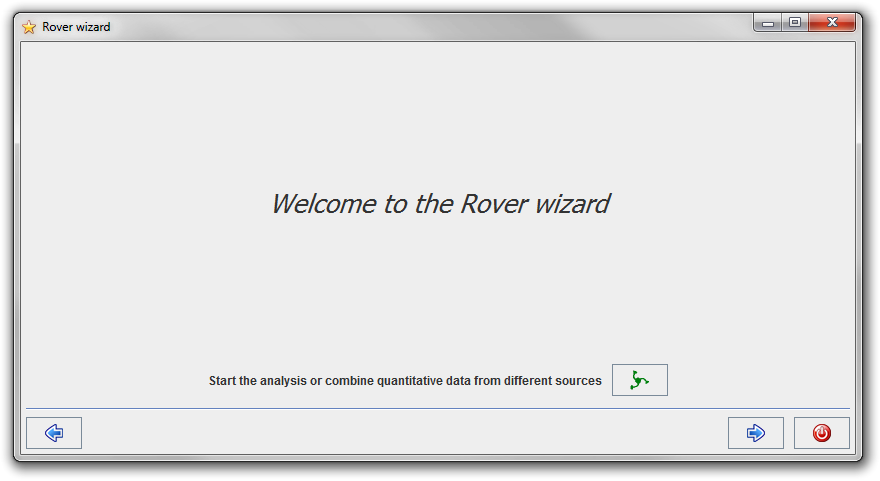
\includegraphics[scale=0.4]{Rover_wizard_S.png}
\caption{The Rover wizard welcome screen}
\label{welcome}
\end{center}
\end{figure}

\begin{figure}[H]
\begin{center}
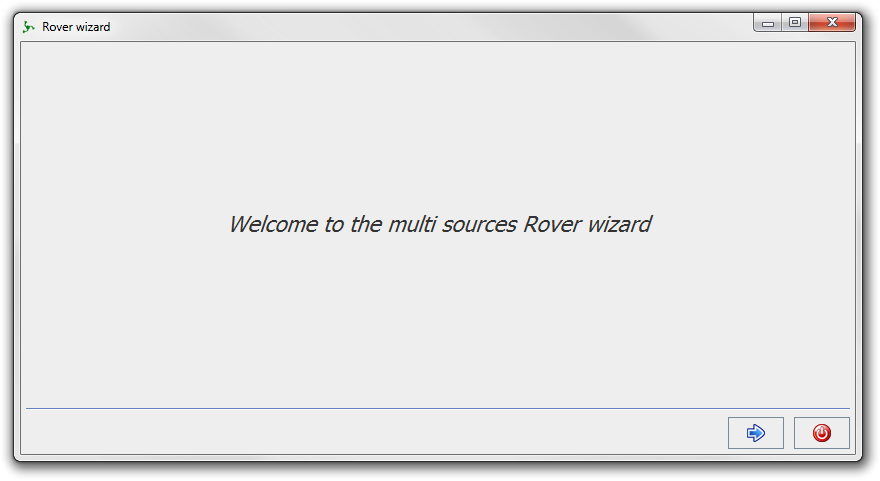
\includegraphics[scale=0.4]{Rover_wizard_M.png}
\caption{The Rover wizard welcome screen for the multiple sources approach}
\label{welcome_M}
\end{center}
\end{figure}

\section{Different steps in the Rover wizard}

\paragraph{}The Rover wizard is a step by step tool for selecting quantitative data and starting the Rover program. This is done by clicking the next 
\includegraphics[scale=0.6, H]{forward.png} and previous 
\includegraphics[scale=0.6, H]{back.png} button at the lower part of the frame.

\subsection{Step 1 - Selection of the information source}

\paragraph{}Rover can load different types of quantitative information from different sources (see figure \ref{step1} and \ref{step1_M} for the multiple sources approach). 

\begin{figure}[H]
\begin{center}
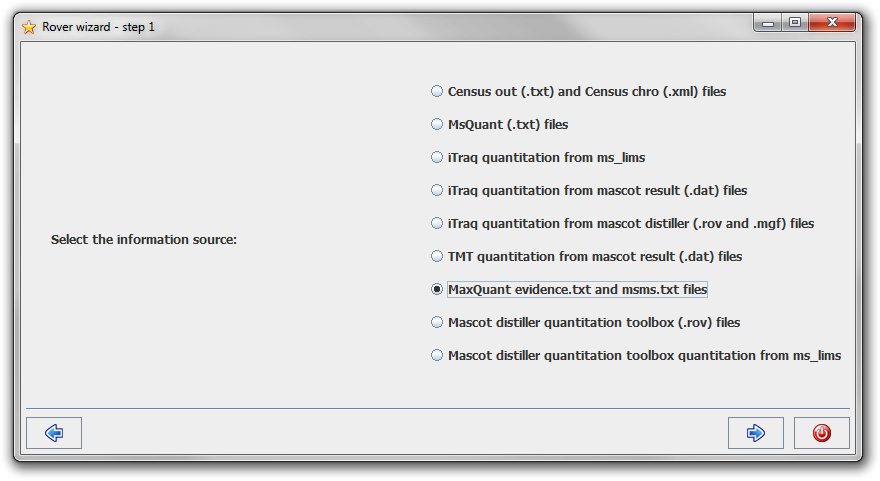
\includegraphics[scale=0.4]{Rover_wizard_-_step_1_S.png}
\caption{Step 1 of the Rover wizard}
\label{step1}
\end{center}
\end{figure}

\begin{figure}[H]
\begin{center}
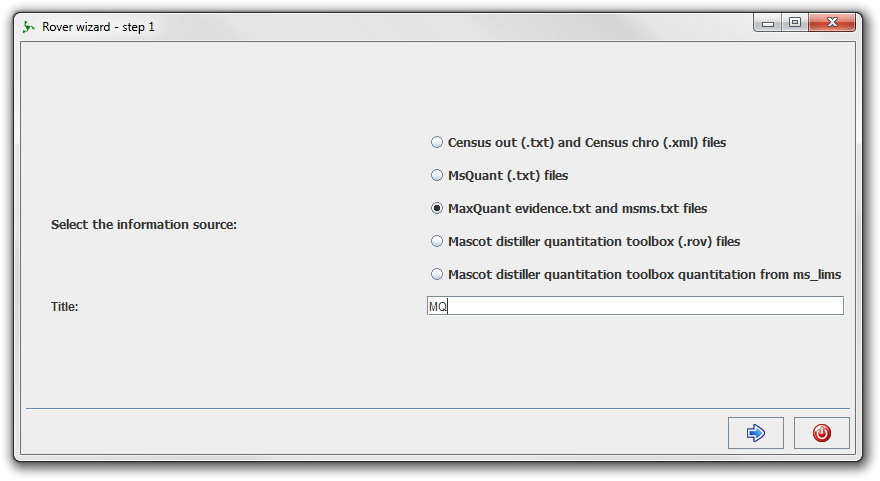
\includegraphics[scale=0.4]{Rover_wizard_-_step_1_M.png}
\caption{Step 1 of the multiple sources Rover wizard. A title has to be given to every set.}
\label{step1_M}
\end{center}
\end{figure}


\paragraph{}Different types of quantitative data can be analysed and viewed by Rover. 
\begin{description}
\item[iTRAQ\texttrademark (isobaric tags for relative and absolute quantitation) data:]The peptides N-terminus is covalently modified by isobaric tags. The quantitative information can be found in the MS/MS spectra. iTRAQ\texttrademark data can be read from \textit{.dat} Mascot result files and from Mascot Distiller \textit{.rov} files. If the information comes from Mascot Distiller, a \textit{.mgf} file must also be given to Rover\footnote{The name of the \textit{.rov} file must start with the name of the \textit{.mgf} file. This \textit{.mgf} file is normally located in the same folder as the \textit{.rov} file.}. 
\item[(Post) metabolic labelled peptides analysed by the Mascot Distiller Quantitation toolbox:]Two or more groups of proteins are metabolically labelled (ex. SILAC labelling, $^{16}$0/$^{18}$0 labelling, \ldots). Quantitative information can be calculated by comparison of the intensities of the precursors in the MS spectra. This comparison is done by the Mascot Distiller Quantitation toolbox. The data are stored in Mascot Distiller \textit{.rov} files. Keep in mind that these \textit{.rov} files must be created with the Quantitation toolbox extension of Mascot Distiller and that the quantitative information and peptide identifications must be stored in the \textit{.rov} file.
\item[SILAC labelling analysed by MaxQuant:]Double and triple SILAC labelled experiments can be analysed by MaxQuant. Two of the MaxQuant result files (msms.txt and evidence.txt) are used by Rover to extract the quantitative information.
\item[MSQuant result files:]MSQuant is a tool for quantitative proteomics/mass spectrometry and processes spectra and LC runs to find quantitative information about proteins and peptides. The quantitative export file (\textit{.txt}) from MSQuant is needed to view MSQuant data in Rover.
\item[Census result files:]Census uses mzXML and DTASelect data for the quantitation of peptides. The output (\textit{.txt}) and chro (\textit{.xml}) files are used as import by Rover.
\end{description}

\paragraph{}Data can be loaded from such files or from ms\_lims. Ms\_lims is a mass-spectrometry focused lims database system (see \url{http://genesis.ugent.be/ms_lims} for more information).  iTRAQ\texttrademark data as well as Mascot Distiller data can be loaded from ms\_lims.

\subsection{Step 2 - Selection of the data}
\subsubsection{From files}
\paragraph{}In the second step the files with quantitative information must be selected . Click the open button (see figure \ref{step2A}) and a file chooser frame appears. Selected the files and click the open button in the file chooser. The selected files will now appear in the selected files list in the wizard frame.

\begin{figure}[H]
\begin{center}
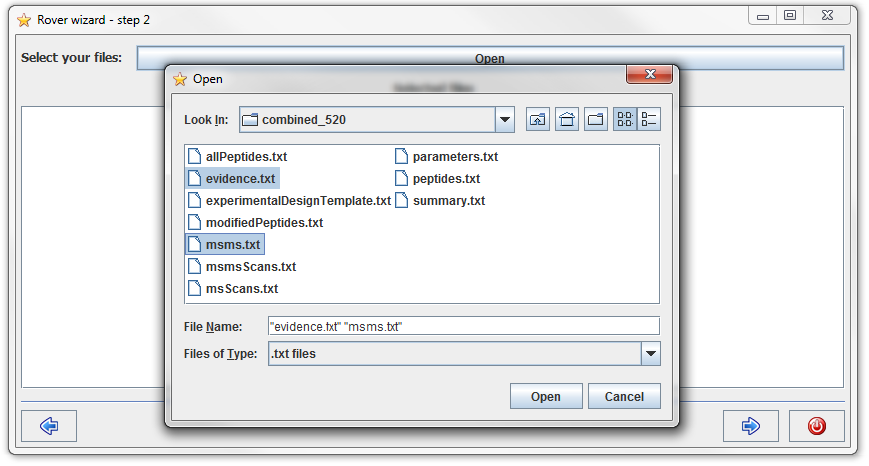
\includegraphics[scale=0.4]{Rover_wizard_-_step_2_S.png}
\caption{Step 2 of the Rover wizard}
\label{step2A}
\end{center}
\end{figure}

\subsubsection{From ms\_lims}
\paragraph{}If a connection to ms\_lims doesn't exist, a frame will appear (see figure \ref{wizardDb}) where a connection to a ms\_lims database can be established.

\begin{figure}[H]
\begin{center}
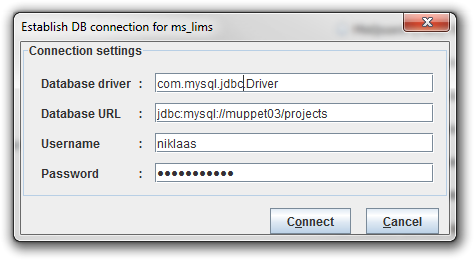
\includegraphics[scale=0.4]{wizardDb.png}
\caption{Frame to make connection to ms\_lims}
\label{wizardDb}
\end{center}
\end{figure}

\paragraph{}If a valid connection is established to ms\_lims, all the project will be loaded in a drop-down menu (see figure \ref{step2B}). If a project is selected, the user, project title, project description, \ldots will be loaded. The selected project will be used as data source in the following steps.

\begin{figure}[H]
\begin{center}
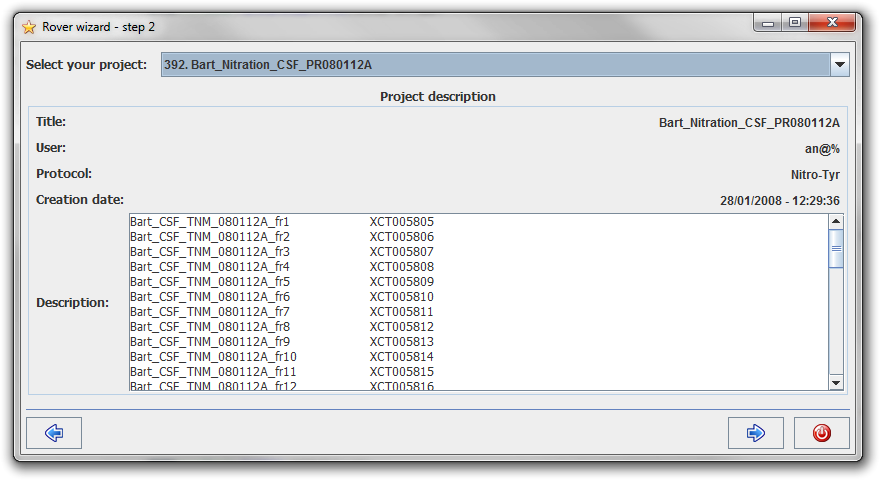
\includegraphics[scale=0.4]{Rover_wizard_-_step_2_DB.png}
\caption{Step 2 of the Rover wizard}
\label{step2B}
\end{center}
\end{figure}

\subsection{Step 3 - Input parameters}
\paragraph{}Several parameters need to be set for Rover in step 3 (see figure \ref{step3}).

\begin{figure}[H]
\begin{center}
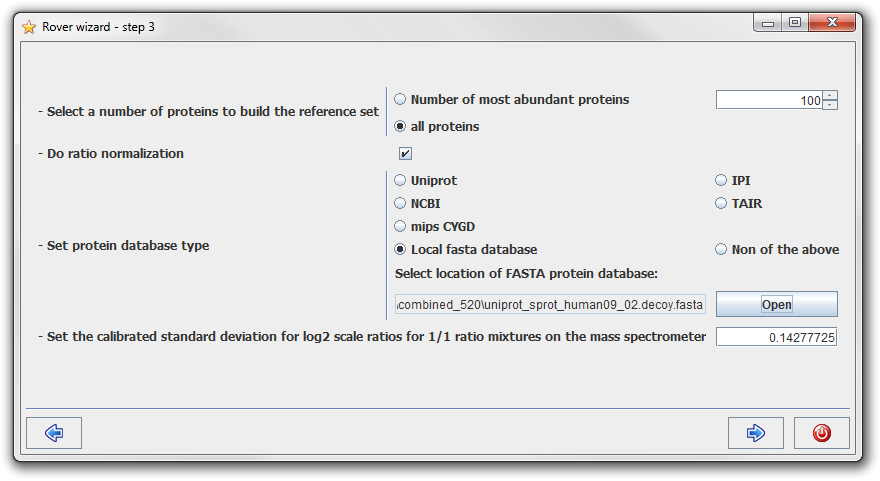
\includegraphics[scale=0.4]{Rover_wizard_-_step_3_S.png}
\caption{Step 3 of the Rover wizard}
\label{step3}
\end{center}
\end{figure}

\subsubsection{Peptide identification confidence level}

\paragraph{}The Mascot peptide identification confidence level (default is 0.99) only needs to be set if data are loaded from files and not from ms\_lims. 

\subsubsection{Reference set}\label{Reference set}

\paragraph{}Rover will create a reference set of proteins. This set will be used to compare protein ratio means. For more information on this reference set, see chapter \ref{Statistics}.

\paragraph{}Two different option exist for creating the reference set. The first option to build the reference set is to use all ratios linked to all proteins. The second option is to use the ratios linked to a specific number (20-300) of the most abundant (based on the number of identified spectra) proteins.

\paragraph{}Rover can be set to take all ratios (valid and invalid) from the selected proteins in the reference set or it can be set to take only the valid ratios. By default rover will take only the valid ratios.

\subsubsection{Database type}\label{Database type}

\paragraph{}Mascot will use a \textit{.fasta} or \textit{.dat} (protein) database on the Mascot server to identify MS/MS spectra. Since Mascot and other file providers don't store protein sequences in their result files, Rover downloads the protein sequences. There are different types of databases and protein accessions supported. Also a local \textit{.fasta} protein database can be selected. The option ``Non of the above" has to be selected if a database was created with user-defined accessions, or if a database was downloaded from an unsupported  source. The protein sequences will not be downloaded for this option. As a result, the protein bar (see \ref{Protein bar}) will not be visualised.

\subsubsection{Instrument standard deviation}\label{Instrument standard deviation}

\paragraph{}Rover will use statistics to calculate the significance of deviation of a ratio value when compared to the reference set. The program will not only use the reference set to create a standard deviation, it will also use the calibrated standard deviation for $\log_{2}$ scale ratios for $\frac{1}{1}$ ratio mixtures measered on a mass spectrometer. More on statistics can be found in chapter \ref{Statistics}.

\paragraph{}A default value of 0.14277725 is given. This was calculated for an Waters Q-TOF Premier in our laboratory.

\subsection{Step 4}
\paragraph{}Step 4 is the final step for the single source method. The Rover wizard will start collecting the data after the start button 
\includegraphics[scale=0.6, H]{finish.png} is clicked (see figure \ref{step4}). Different steps are performed before everything is loaded and visualized (see \ref{dataViewing}). During the loading process a window will appear (see figure \ref{step7_2}) where the  not regulated component and the expected ratio median must be set for every ratio. 

\begin{figure}[H]
\begin{center}
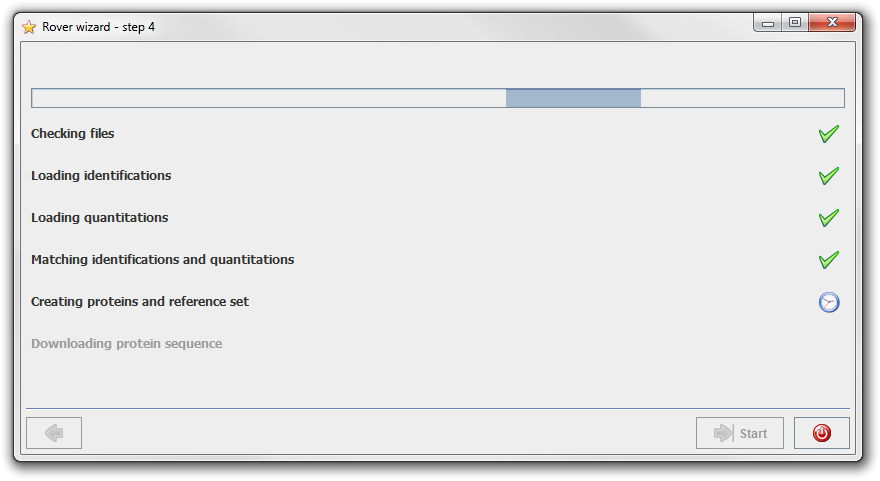
\includegraphics[scale=0.4]{Rover_wizard_-_step_4_S.png}
\caption{Step 4 of the Rover wizard}
\label{step4}
\end{center}
\end{figure}

\begin{itemize}
\item If the loaded data come from files, these files will be checked if they exist and if they have the correct quantitative information
\item The peptide identifications will be loaded for every file
\item The quantitative information will be loaded for every file
\item The peptide identifications will be linked to the quantitative information for every file
\item Different peptides are grouped to proteins and a reference set is created. 
\item The protein sequences will be downloaded if possible.
\end{itemize}

\paragraph{}If the multiple sources approach is used a second source (see figure \ref{step4_M}) can be added and this takes the wizard back to step 1 (data type selection step).

\begin{figure}[H]
\begin{center}
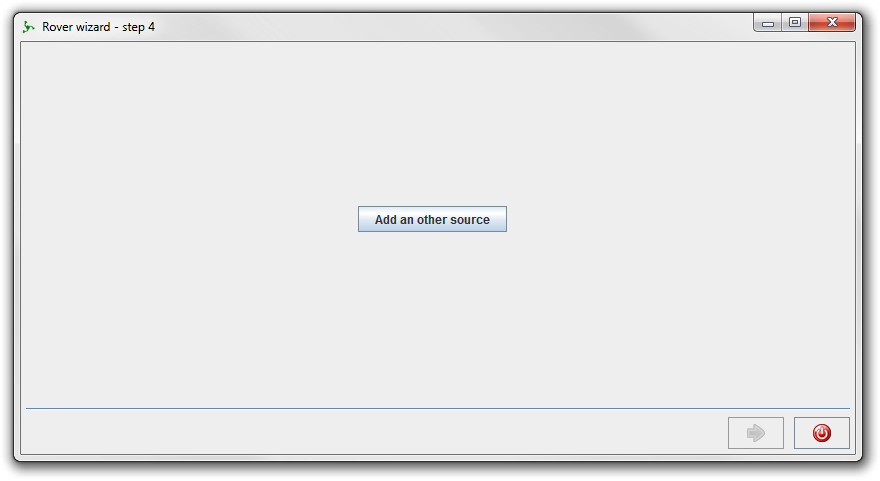
\includegraphics[scale=0.4]{Rover_wizard_-_step_4_M.png}
\caption{Step 4 of the multiple sources Rover wizard}
\label{step4_M}
\end{center}
\end{figure} 

\subsection{Step 5 - Data retrieval (only multiple sources approach)}
\paragraph{}The Rover wizard will collect the data from the different sources (see figure \ref{step5}). 

\begin{figure}[H]
\begin{center}
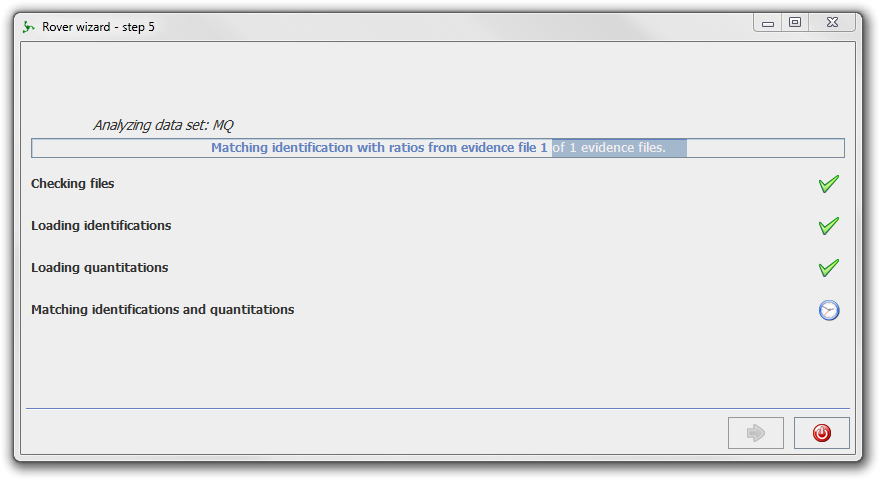
\includegraphics[scale=0.4]{Rover_wizard_-_step_5_M.png}
\caption{Step 5 of the Rover wizard}
\label{step5}
\end{center}
\end{figure}

\subsection{Step 6 - Grouping ratios (only multiple sources approach)}
\paragraph{}The different ratios from the different sources must be linked to each other. This step is necessary because the correct ratios from different source must be merged. The common ratio name must be set by filling in the text box (see figure \ref{step6_1}). The ratios from the other sources can now be linked to this common ratio by selecting it in the list (see figure \ref{step6_2}). Ratios can in this step be selected for inversion. This could be necessary if L/H ratios must be merged with H/L ratios.

\begin{figure}[H]
\begin{center}
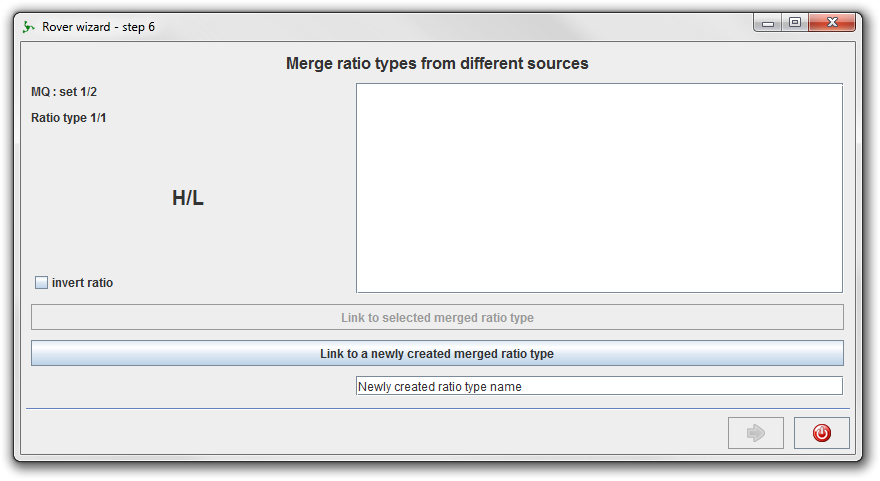
\includegraphics[scale=0.4]{Rover_wizard_-_step_6_1.png}
\caption{Step 6.1 of the Rover wizard}
\label{step6_1}
\end{center}
\end{figure}


\begin{figure}[H]
\begin{center}
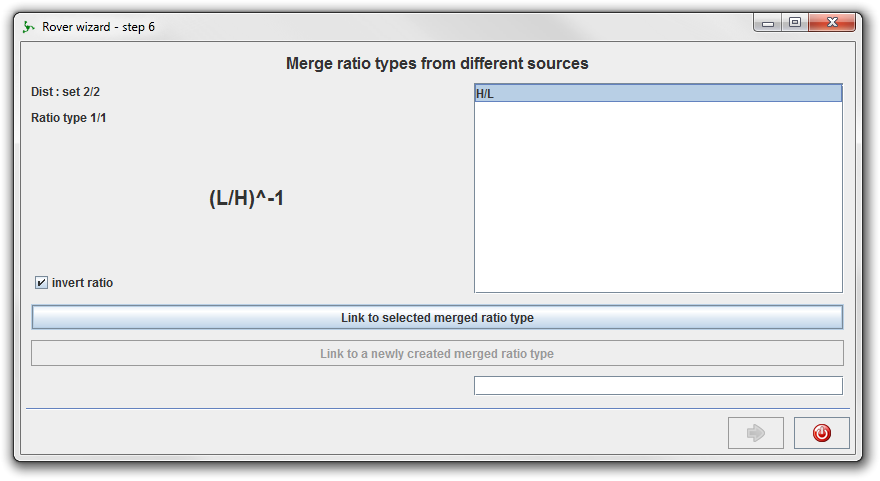
\includegraphics[scale=0.4]{Rover_wizard_-_step_6_2.png}
\caption{Step 6.2 of the Rover wizard}
\label{step6_2}
\end{center}
\end{figure}

\subsection{Step 7 - Grouping components (only multiple sources approach)}
\paragraph{}Just like in step 6, the different components from the different sources must be merged (see figure \ref{step7}). When the different components are linked a window will appear (see figure \ref{step7_2}) where the the not regulated component and the expected ratio median must be set for every ratio from every source. 

\begin{figure}[H]
\begin{center}
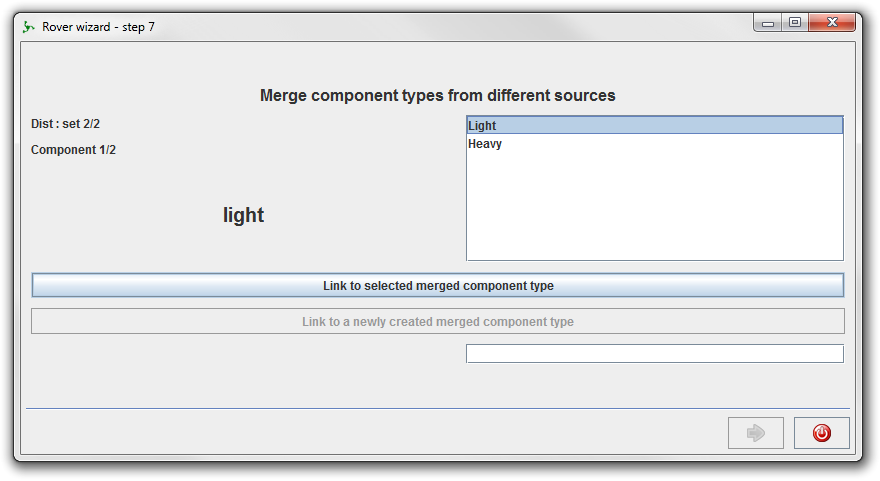
\includegraphics[scale=0.4]{Rover_wizard_-_step_7.png}
\caption{Step 7.1 of the Rover wizard}
\label{step7}
\end{center}
\end{figure}

\begin{figure}[H]
\begin{center}
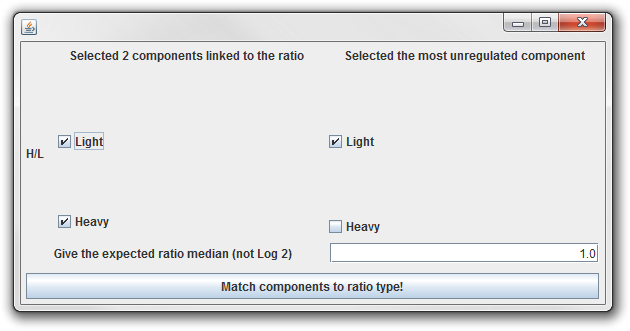
\includegraphics[scale=0.4]{matcher_S.png}
\caption{Step 7.2 of the Rover wizard}
\label{step7_2}
\end{center}
\end{figure}

\subsection{Step 8 - Data merging}
\paragraph{}The data from the different sources will be merged. This can only be done after a location and scale normalization process.  

\begin{figure}[H]
\begin{center}
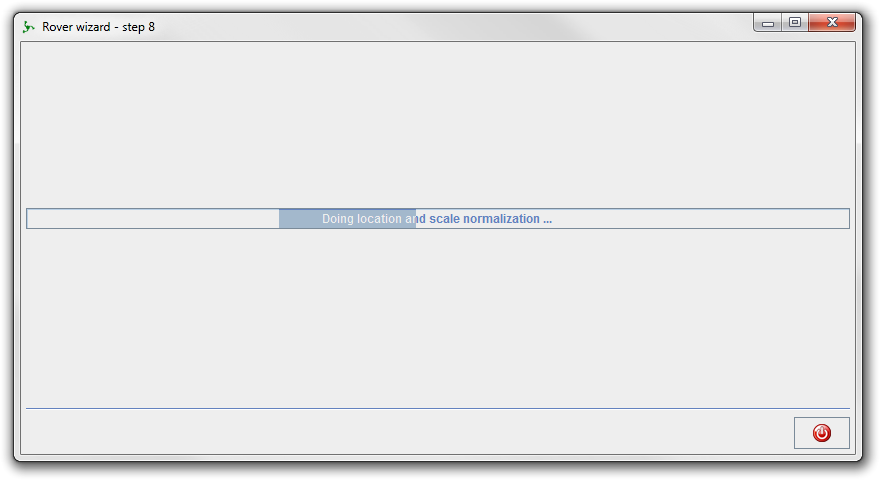
\includegraphics[scale=0.4]{Rover_wizard_-_step_8.png}
\caption{Step 8 of the Rover wizard}
\label{step8}
\end{center}
\end{figure}


%chapter on viewing the data
\chapter{Data viewing with Rover} \label{dataViewing}
\section{Overview}
\paragraph{}After all the different steps in the Rover wizard are executed the main Rover frame will be shown. This frame (figure \ref{roverGui}) consists of different panels, which will be explained in the following sections. These visualize the data in different ways and from different angles, making it easier for the user to validate a (regulated) protein. To tackle the problem of peptides pointing to multiple proteins in a data search space (protein inference), Rover uses color labels for individual peptides: peptides unique for a protein accession are labelled blue, peptides belonging to multiple protein accessions are labelled orange and Occam's razor peptides are labelled red in every panel. In this way, Rover clearly indicates which peptides are shared between different protein accessions and are thus prone to influence protein ratios in a unwanted way. 
\begin{figure}[H]
\begin{center}
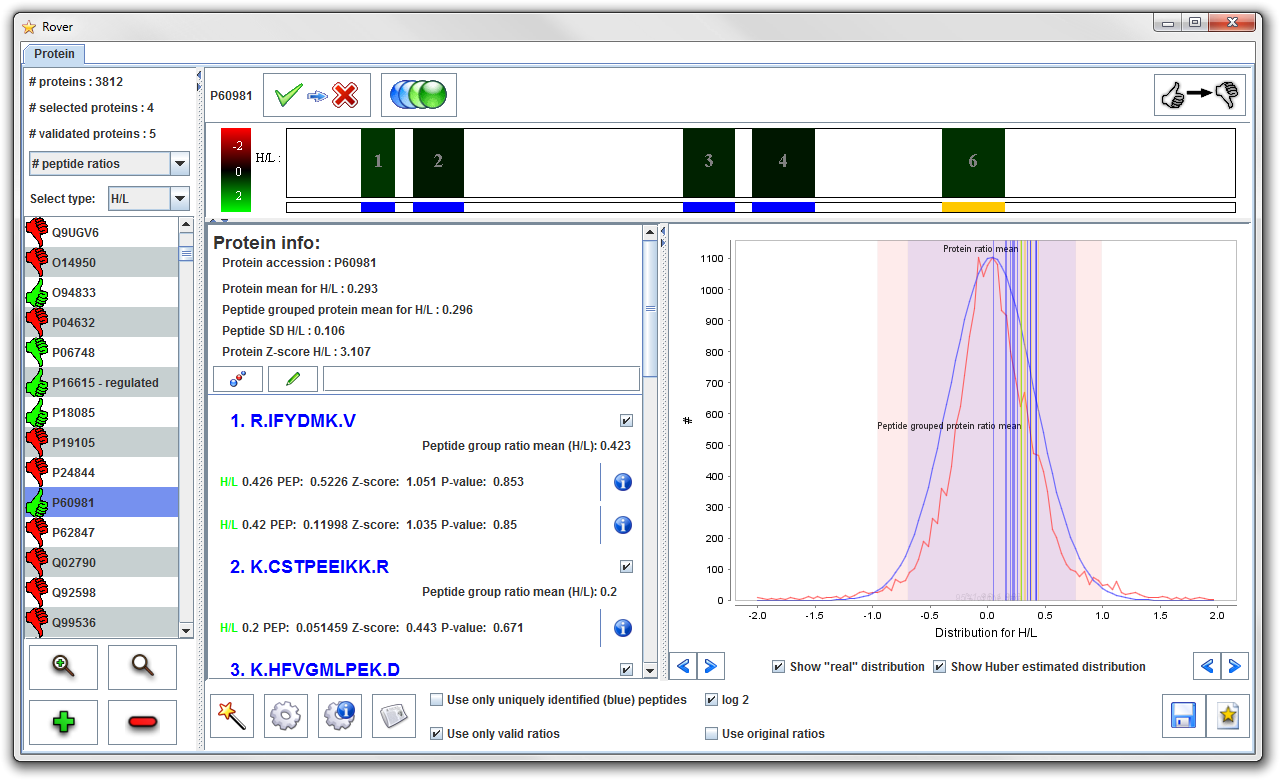
\includegraphics[scale=0.4]{Rover_S.png}
\caption{The main Rover frame}
\label{roverGui}
\end{center}
\end{figure}

\begin{figure}[H]
\begin{center}
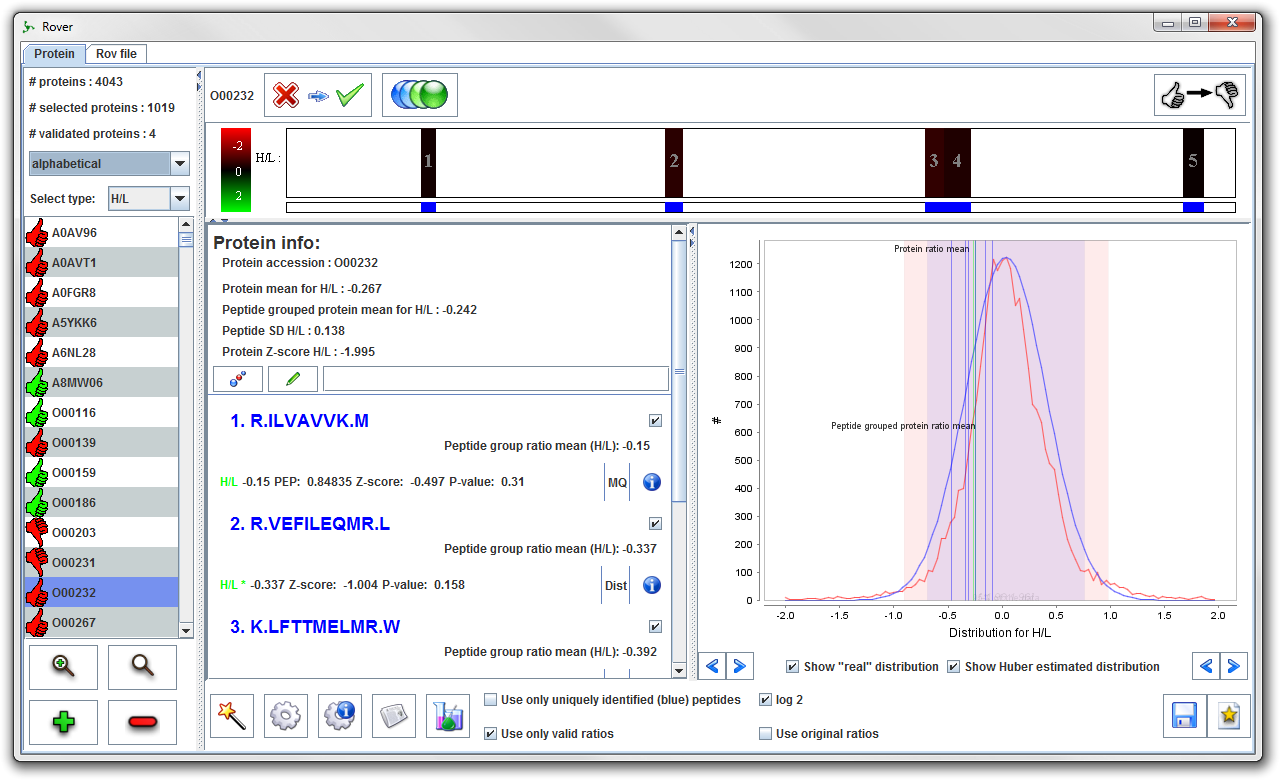
\includegraphics[scale=0.4]{Rover_M.png}
\caption{The main multiple sources Rover frame}
\label{roverGuiMulti}
\end{center}
\end{figure}

%%%%%%%%%%%%%%%%%%
% PROTEIN LIST
%%%%%%%%%%%%%%%%%%
\section{Protein list panel}\label{Protein list}

\paragraph{}A list with all the proteins (identified by their protein accessions) that were found in the input data is displayed on the left side of the main Rover frame (see figure \ref{roverGui}). When a filter (see section \ref{filter}) is applied, only the filtered proteins will be displayed. Four different icons display the status of each protein. This protein status indicates if a user selected an interesting protein (selected status) and if a user indicated that a protein has been validated (validated status).

\begin{itemize}
\item 
\includegraphics[scale=0.6, H]{thumbsDownRed.png} The protein is \textit{not selected} and \textit{not validated}.
\item 
\includegraphics[scale=0.6, H]{thumbsUpRed.png} The protein is \textit{selected} and \textit{not validated.}
\item 
\includegraphics[scale=0.6, H]{thumbsDownGreen.png} The protein is \textit{not selected} and \textit{validated}.
\item 
\includegraphics[scale=0.6, H]{thumbsUpGreen.png} The protein is \textit{selected} and \textit{validated}.
\end{itemize}

\paragraph{}At the top of the protein list panel three numbers indicate the total number of proteins, the number of selected proteins and the number of validated proteins. Also the proteins can be sorted in different order by choosing a sorting type and ratio just below these numbers.

\paragraph{}At the bottom of the protein list panel are four buttons.

\begin{itemize}		
\item 
\includegraphics[scale=0.6, H]{viewAll.png} When this button is clicked \emph{all the proteins} will be displayed in the protein list.
\item 
\includegraphics[scale=0.6, H]{viewSelection.png} When this button is clicked \emph{the selected proteins} will be displayed in the protein list.
\item 
\includegraphics[scale=0.6, H]{plus.png} When this button is clicked all the \emph{proteins in the protein list} will be \emph{selected}.
\item 
\includegraphics[scale=0.6, H]{min.png} When this button is clicked all the \emph{proteins in the protein list} will be \emph{unselected}.
\end{itemize}

%%%%%%%%%%%%%%%%%%
% PROTEIN BAR
%%%%%%%%%%%%%%%%%%
\section{Protein bar}\label{Protein bar}

\paragraph{}The protein bar (see figure \ref{barGui}), which is located at the top of the main Rover frame (see figure \ref{roverGui}), visualizes the protein coverage and the peptide ratios. Rover will only show the peptides and ratios that are used for the calculation of the protein mean. Thus, if Rover is in the ``\textit{show only valid peptides}" mode, only the peptides with a valid peptide ratio will be displayed in the protein bar.

\begin{figure}[H]
\begin{center}
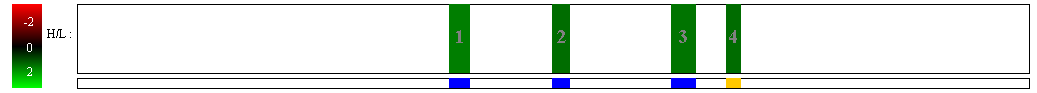
\includegraphics{proteinBar.png}
\caption{The protein bar}
\label{barGui}
\end{center}
\end{figure}

\paragraph{}A color gradient box on the left side of this panel shows a gradient from red to green between the minimum and maximum ratio values. This minimum and maximum can be changed by changing the width of the ratio distribution graph (see section \ref{ratio distribution graph}).

\paragraph{}The black rectangle represents the protein. On this rectangle, the peptides with their corresponding positions in the protein are shown. The number in the peptide box corresponds to the peptide group with the same number in the protein panel (see section \ref{proteinInfoPanel}). The length of these peptide boxes correlates with the actual peptide length normalised to the protein length. The color of the peptide box reflects the peptide ratio (if the same peptide is identified more than once, the ratio mean will be used). If multiple ratios were calculated (ex. iTRAQ \textrademark) for the peptides, multiple rectangles will be shown.

\paragraph{}At the bottom of this panel there is a small bar with blue, orange and red boxes. The blue boxes show the position of peptides (with valid and invalid ratios) that are uniquely linked to this protein. Orange boxes reflect the position of peptides (with valid and invalid ratios) that can be linked to multiple proteins.

%%%%%%%%%%%%%%%%%%
% FILTER
%%%%%%%%%%%%%%%%%%
\section{Filter}\label{filter}
\paragraph{}Not all the proteins must be validated. With the filter tool, proteins of interest or peptides with a specific ratio can be selected. After a filter step is performed, Rover will show how many proteins it has filtered and it will present these in the protein list (see section \ref{Protein list}).

\paragraph{}Different filters were created to select a specific subset of proteins. There are generally two types of filters. Filters that will filter on the peptide (ratio) level and filters that will filter on the protein level. Filters that work on the peptide level can be set to only use peptides with a valid ratio or uniquely identified peptides.

\begin{figure}[H]
\begin{center}
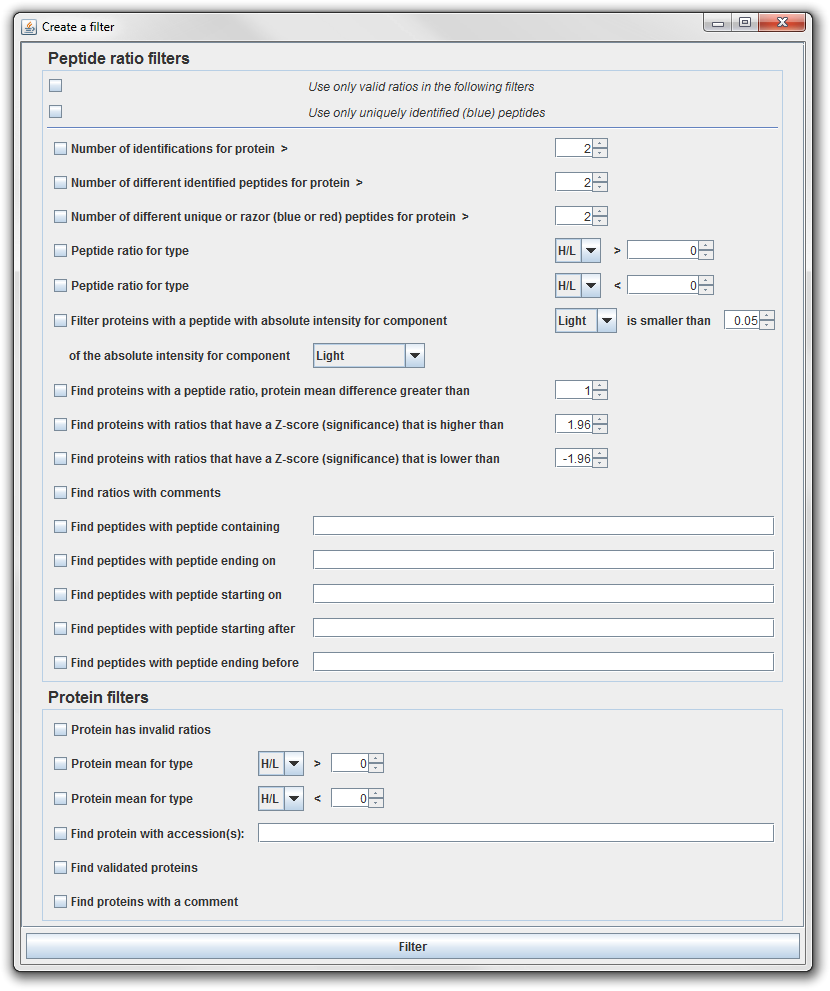
\includegraphics[scale=0.4]{Filter_S.png}
\caption{The filter panel}
\end{center}
\end{figure}
\\
\textbf{Number of identifications for protein \textgreater \ $\bigstar$}
\begin{quotation}
A protein will be filtered if more than $\bigstar$ peptides are linked to this protein.
\end{quotation}
\\
\textbf{Number of different identified peptides for protein \textgreater \ $\bigstar$}
\begin{quotation}A protein will be filtered if more than $\bigstar$ different peptides are linked to this protein.
\end{quotation}
\\
\textbf{Peptide ratio for type A \textgreater \ $\bigstar$}
\begin{quotation}A protein will be filtered if one of the peptide ratio means for A is larger than $\bigstar$.
\end{quotation}
\\
\textbf{Peptide ratio for type A \textless \ $\bigstar$}
\begin{quotation}A protein will be filtered if one of the peptide ratio means for A is smaller than $\bigstar$.
\end{quotation}
\\
\textbf{Filter proteins with a peptide with absolute intensity for component A \\ is smaller than $\bigstar$ of the absolute intensity for component B}
\begin{quotation}A protein will be filtered if the absolute intensity for A is $\bigstar$ times the absolute intensity of B. This filter only works if the data are from the Mascot Distiller Quantitation toolbox.
\end{quotation}
\\
\textbf{Find proteins with a peptide ratio, protein mean difference greater than: $\bigstar$}
\begin{quotation}A protein will be filtered if a difference between a peptide ratio and protein mean is larger than $\bigstar$.
\end{quotation}
\\
\textbf{Find proteins with ratio that have a Z-score (significance) that is higher than: $\bigstar$}
\begin{quotation}A protein will be filtered if a significance of a peptide ratio is larger than $\bigstar$. See chapter \ref{Statistics} for more information on the significance.
\end{quotation}
\\
\textbf{Find proteins with ratio that have a Z-score (significance) that is lower than: $\bigstar$}
\begin{quotation}A protein will be filtered if a significance of a peptide ratio is smaller than $\bigstar$. See chapter \ref{Statistics} for more information on the significance.
\end{quotation}
\\
\textbf{Find ratios with comments}
\begin{quotation}A protein will be filtered if one of the peptide ratios that is linked to the protein has a comment made by a Rover user.
\end{quotation}
\\
\textbf{Find peptides with peptide containing $\bigstar$}
\begin{quotation}A protein will be filtered if one of the peptides contains the $\bigstar$ sequence.
\end{quotation}
\\
\textbf{Find peptides with peptide ending on $\bigstar$}
\begin{quotation}A protein will be filtered if one of the peptides ends on $\bigstar$.
\end{quotation}
\\
\textbf{Find peptides with peptide starting on $\bigstar$}
\begin{quotation}A protein will be filtered if one of the peptides starts with $\bigstar$.
\end{quotation}
\\
\textbf{Find peptides with peptide starting after $\bigstar$}
\begin{quotation}A protein will be filtered if one of the peptides starts after $\bigstar$.
\end{quotation}
\\
\textbf{Find peptides with peptide ending before $\bigstar$}
\begin{quotation}A protein will be filtered if one of the peptides ends before $\bigstar$.
\end{quotation}
\\
\textbf{Find peptides with N-terminal modification $\bigstar$}
\begin{quotation}A protein will be filtered if one the N-terminal modifications equals $\bigstar$. (This filter can only be used when the data comes from Mascot Distiller)
\end{quotation}
\\
\textbf{Protein has invalid ratios}
\begin{quotation}A protein will be filtered if one of the peptide ratios that is linked to the protein is invalid.
\end{quotation}
\\
\textbf{Protein mean for type A \textgreater \ $\bigstar$}
\begin{quotation}}A protein will be filtered if the protein mean for A is larger than $\bigstar$.
\end{quotation}
\\
\textbf{Protein mean for type ratiotype \textless \ $\bigstar$}
\begin{quotation}A protein will be filtered if the protein mean for ratiotype (ex. L/H) is smaller than $\bigstar$.
\end{quotation}
\\
\textbf{Find protein with accession: $\bigstar$}
\begin{quotation}A protein will be filtered if the protein accession equals $\bigstar$. Multiple accessions separated by commas are also valid as an input parameter.
\end{quotation}
\\
\textbf{Find validated proteins}
\begin{quotation}A protein will be filtered if it is validated.
\end{quotation}
\\
\textbf{Find proteins with a comment}
\begin{quotation}A protein will be filtered whenever it has a protein comment.
\end{quotation}
\\

%%%%%%%%%%%%%%%%%%
% Ratio distribution graph
%%%%%%%%%%%%%%%%%%
\section{Ratio distribution graph}\label{ratio distribution graph}

\paragraph{}In the ratio distribution graph both the peptide ratios of the selected protein and the ratios in the reference set (see section \ref{Reference set}) are shown. The distribution in the reference set can be visualized in two different ways.

\begin{itemize}
\item The first way is the ``real" distribution. The ratios of the reference set are used to create a histogram. The red background spans 95\% ([2.5 \%; 97.5 \%]) of all data.
\item The second way is the ``Huber" estimated distribution. The ratios of the reference set are used to calculate an average and a standard deviation ($\sigma$). These are used to create a distribution (see chapter \ref{Statistics} for more information). The blue background is the 95\% confidence interval [-1.96 $\sigma$; 1.96 $\sigma$].
\end{itemize}

\paragraph{}The blue, orange and red vertical lines in the graph are the peptide ratios linked to the selected protein. These are blue when the peptide is only linked to this protein, orange when the peptide is linked to multiple proteins and red when the peptide is an Occam's razor peptide. Two green lines show the ``\textit{Protein ratio mean}" and the ``\textit{Peptide grouped protein ratio mean}".

\paragraph{}At the bottom of the ratio distribution graph are check buttons to choose which of the distribution presentations are visualized. There are also buttons to change the width of the graph.

%%%%%%%%%%%%%%%%%%
% Protein panel
%%%%%%%%%%%%%%%%%%
\section{Protein panel}\label{proteinInfoPanel}

\paragraph{}The protein panel is located at the left side of the ratio distribution graph in the main Rover frame (see figure \ref{roverGui}). The ``\textit{protein mean}" and the``\textit{peptide grouped protein mean}" are at the top of the protein info panel. The ``\textit{peptide grouped protein mean}" is the mean of all the peptide groups ratio means (the mean ratio of all the peptides with the same identified sequence). The ``\textit{protein mean}" is the mean of all peptide ratios. Sometimes some peptide ratios will be excluded in the calculation of the protein mean. This can happen when only valid or unique peptides are used in the calculation. This usage can be set by two check boxes on the lower button panel (see \ref{lowerButtonPanel}). The ``\textit{Peptide SD}" is the standard deviation calculated for all the ratios used in the protein ratio calculation. The ``\textit{Protein Z-score}" is the Z-score calculated for the protein ratio based on the reference set median and standard deviation ($\sigma$) and the number of the ratios (n) used in the protein ratio calculation (see formula \ref{zscore}).

\begin{equation}
Z-score = \dfrac{Protein \ ratio - Reference \ set \ median}{\frac{Reference \ set \ \sigma}{\sqrt{n}}}
\label{zscore} 
\end{equation}

\paragraph{}A comment can be given to a protein by typing it in the comment text field and by clicking the comment button 
\includegraphics[scale=0.6, H]{pencil.png}. This comment will append the name (= accession) of the protein. This name can be seen in the protein list (see \ref{Protein list}) and in the top button panel (see \ref{Top button panel}).

\paragraph{}MS/MS spectra that identify the same peptide are grouped under this peptide sequence in peptide groups. If the peptide sequence can be matched on the protein sequence the amino acid before and after the peptide will also be given before and after the identified peptide sequence (seperated by a ``."). The colour of the peptide sequence is orange if this peptide is linked to multiple proteins, blue when the peptide is only be linked to the selected protein and red when the peptide is an Occam's razor peptide. When the mouse is hovered over an orange and red peptides a small box with the accessions of the proteins to which it is linked, appears.

\paragraph{}Whenever the peptide sequence from one peptide group is clicked it will show or hide (depending on the visualization status) all the ratio groups that are linked to this peptide group. All the ratio groups can be hidden by clicking 
\includegraphics[scale=0.6, H]{hide.png} or can be revealed again by clicking 
\includegraphics[scale=0.6, H]{show.png}.

\paragraph{}Every peptide identification is linked to a ratio group. A ratio group has more than one ratio, if more than one ratio type is calculated (ex. L/H, M/H and L/M). At the right side of this ratio group there is a ``\textit{more information}" 
\includegraphics[scale=0.6, H]{info.png} button. When this button is clicked, the more info panel is shown (see \ref{moreInfo}).

\paragraph{}If the ratio is invalid, the ratio value is in red and the ratio quality is shown (only with Mascot Distiller Quantitation toolbox data). If the Mascot Distiller Quantitation toolbox has reasons to set the ratio invalid it will be shown there. The ratio is green if it's a valid ratio. The Z-score is the number of standard deviations that corresponds with the difference between the ratio and the reference set ratio mean (see section \ref{Reference set} and chapter \ref{Statistics}) The P-value is calculated with this Z-score. The ratio comment (if any) will be shown below the ratio in italics.


\paragraph{}If Rover is run in the multiple sources mode, the title of the source will be indicated left to the ``\textit{more information}" 
\includegraphics[scale=0.6, H]{info.png} button. If a ratio is inverted in the combination process the name will of the ratio will be appended by * (see figure \ref{roverGuiMulti} for an example).


\paragraph{}If one of the peptides groups is not to be used to calculate a protein mean it can be deselected by clicking the check box next to the peptide sequence. This will also hide the ratios from the distribution graph (see \ref{ratio distribution graph}) and the peptide box from the protein bar (see \ref{Protein bar}).


%%%%%%%%%%%%%%%%%%
% More info panel
%%%%%%%%%%%%%%%%%%
\section{More info panel} \label{moreInfo}

\paragraph{}In this panel (see figure \ref{moreInfoPanel}) the ratio can be commented and set (in)valid. If the data are loaded from ms$\_$lims, this comment and valid change will be directly stored in ms$\_$lims. Otherwise, this can be stored in a \textit{.ROVER} file (see section \ref{save panel}). 

\paragraph{}More information concerning the peptide identification (score, mass, modified peptide, \ldots) is shown on this panel.

\paragraph{}If Mascot Distiller Quantititation toolbox data is loaded, the correlation and fraction for this peptide group is given on the top of the panel. An XIC graph and a bar chart with absolute intensities is also shown. The pink area on the XIC graph shows the scans that the Quantitation toolbox used to calculate the ratio.

\paragraph{}If MaxQuant data is loaded a bar chart with absolute intensities is visualized. 

\begin{figure}[H]
\begin{center}
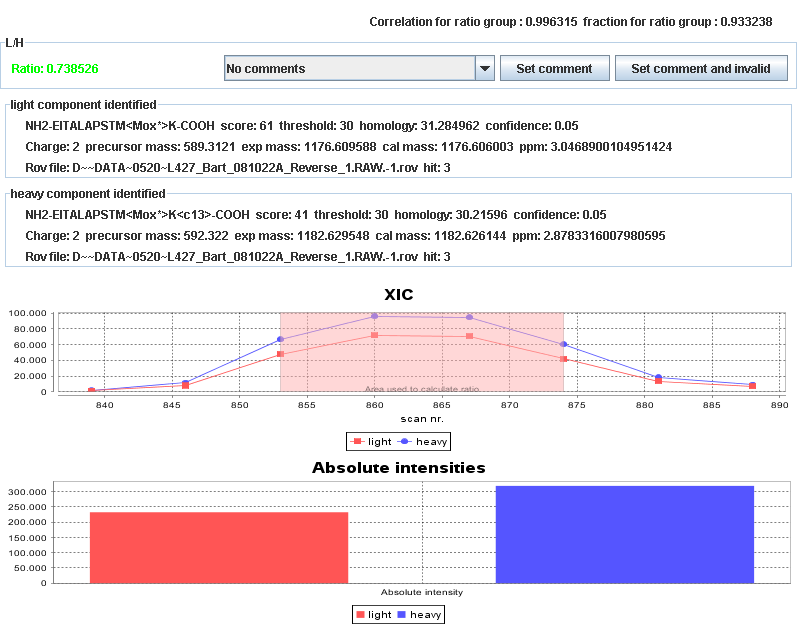
\includegraphics[scale=0.7]{moreinfopanel.png}
\caption{This is an example of a ``more info" panel that displays data loaded from Mascot Distiller Quantitation toolbox files.}
\label{moreInfoPanel}
\end{center}
\end{figure}

%%%%%%%%%%%%%%%%%%
% More info panel
%%%%%%%%%%%%%%%%%%
\section{Button panels}
\subsection{Top button panel}\label{Top button panel}

\paragraph{}The buttons on the top panel relate to the selected protein

\begin{itemize}
\item 
\includegraphics[scale=0.6, H]{setValidated.png} When this button is pushed the protein will be given a \textit{validated} status. 
\item 
\includegraphics[scale=0.6, H]{setNotValidated.png} When this button is pushed the protein will be given a \textit{not validated} status.
\item 
\includegraphics[scale=0.6, H]{homepage.png} When this button is pushed the default internet browser will be opened to the website (if available) describing this protein.
\item 
\includegraphics[scale=0.6, H]{isoform.png} When this button is pushed the possible \textit{isoforms} (proteins with peptides that can be linked to two or more proteins) will be loaded in the protein list (see section \ref{Protein list}).
\item 
\includegraphics[scale=0.6, H]{addSelection.png} When this button is pushed the protein will be \textit{selected}.
\item 
\includegraphics[scale=0.6, H]{deleteSelection.png} When this button is pushed the protein will be \textit{deselected}.
\end{itemize}

\subsection{Lower button panel}\label{lowerButtonPanel}

\paragraph{}The buttons at the lower end have general functions.
\begin{itemize}
\item 
\includegraphics[scale=0.6, H]{wizard.png} When this button is pushed the filter panel appears (see section \ref{filter}).
\item 
\includegraphics[scale=0.6, H]{misc.png} When this button is pushed a small panel appears where the protein reference set can be adapted (see section \ref{Reference set}).
\item 
\includegraphics[scale=0.6, H]{misc_info.png} When this button is pushed a small panel appears with information concerning the protein reference set. The number of proteins and ratios used in the reference set as well as the standard deviation and mean calculated with the reference set will be listed in this panel. The exact limits of the 95\% confidence interval [-1.96 $\sigma$; 1.96 $\sigma$] and the data limits [2.5\%, 97.5\%] are given for every ratio type.
\item 
\includegraphics[scale=0.6, H]{log.png} When this button is pushed a small panel appears with a log. In this log you can see how many proteins were filtered, the protein that was validated, deselected, \ldots .
\item \includegraphics[scale=0.6, H]{edu_science.png} When this button is pushed (only available if the loaded data are Mascot Distiller Quantitation toolbox data) all the ratio groups of the selected protein will be grouped by \textit{.rov} file and \textit{hit} and will be put in a list on a second tab. When one ratio group is selected the ``\textit{more information panel}" is shown (see \ref{moreInfo}). In this tab, the ratio groups with invalid ratios can be selected by clicking the ``\textit{show only invalid ratios}" check box at the bottom of the tab.
\item \includegraphics[scale=0.6, H]{filesave.png} When this button is pushed the save/export panel appears (see \ref{save panel}).
\item \includegraphics[scale=0.6, H]{rover.png} When this button is pushed selected proteins and information on peptide ratios, ratio comments, \ldots will be loaded from a \textit{.ROVER} file.
\item A check box controls the state (\log$_{2}$ or normal value peptide ratios) of the calculated and visualized ratio.  
\item A check box controls the state of the ``\textit{Use only uniquely identified (blue) peptides}".
\item A check box controls the state of the ``\textit{use only valid peptide ratios}".
\item A check box controls the state of the ``\textit{use original ratios}". If this is checked the original ratios will be used in the calculations and not the location and scale normalized ones. This is only available in the multiple sources approach.
\end{itemize}

%%%%%%%%%%%%%%%%%%
% Export panel
%%%%%%%%%%%%%%%%%%
\section{Export panel}\label{save panel}
\paragraph{}Different types of export can be choosen on the export panel (see figure \ref{export panel}). Also, the user can choose which proteins will be exported. \textit{All} proteins, the \textit{selected} proteins, the \textit{validated} proteins or the \textit{previously viewed} protein can be choosen.
\begin{itemize}
\item  \includegraphics[scale=0.6, H]{pdf.png} When this button is pushed, the protein bar (see \ref{Protein bar}), the ratio distribution graph (see \ref{ratio distribution graph}) and the information in the protein panel (see \ref{proteinInfoPanel}}) will be written in a \textit{.PDF} file for every protein selected for export.
\item  \includegraphics[scale=0.6, H]{csv.png} When this button is pushed information for every ratio group from every protein selected for export will be written in an excel viewable \textit{.CSV} file. 
\item  \includegraphics[scale=0.6, H]{csv_protein.png} When this button is pushed information for every protein selected for export will be written in an excel viewable \textit{.CSV} file.
\item  \includegraphics[scale=0.6, H]{rover.png} When this button is pushed a \textit{.ROVER} file will be written. In a \textit{.ROVER} file the user adjusted data will be stored\footnote{If quantitative data from ms\_lims are loaded, the ratio status and ratio comment will be stored in the database. }. Five types of user adjustable data exist.
\begin{itemize}
\item The ratio status can be set valid or invalid.
\item A comment can be given to a ratio
\item A protein can be set selected and validated
\item Peptide groups (peptide with the same peptide identification) can be excluded in the protein mean calculation.
\item A comment can be given to a protein.
\end{itemize}
\end{itemize}


\begin{figure}[H]
\begin{center}
\includegraphics[scale=0.4]{save_panel.png}
\caption{The export panel}
\label{export panel}
\end{center}
\end{figure}


%%%%%%%%%%%%%%%%%%
% Statistics
%%%%%%%%%%%%%%%%%%
\chapter{Statistics}\label{Statistics}

\paragraph{}Statistics are used to compare and review the peptide ratios from the selected proteins with the peptide ratios from a reference set. This reference set is a number (20-300) of the most abundant proteins or are all proteins found in the data (see section \ref{Reference set}).

\paragraph{}Robust statistics is used to correct for the effect of outliers on the average and standard deviation ($\sigma$). Not the mean but the median is used as the average \log $_{2}$ peptide ratio value for the reference set. The standard deviation is used as measure of the variability of the \log $_{2}$ peptide ratios in the reference set.

\paragraph{}The standard deviation is calculated by a Huber's M-estimation. The \log $_{2}$ peptide ratios will be transformed by a process called winsorisation. In this process, the \log $_{2}$ peptide ratios with a value (see formula \ref{winsor1} and \ref{winsor2}) will be changed in \ref{winsor3} and \ref{winsor4} respectively.

\begin{equation}
\log _{2} (peptide \ ratio) \ \textless  \ median - 1.5 \  \sigma  \ (of  \  the  \ previous \  winsorization)
\label{winsor1} 
\end{equation}
\begin{equation}
\log _{2} (peptide \ ratio) \  \textgreater  \ median + 1.5 \  \sigma  \ (of  \ the  \ previous \  winsorization)
\label{winsor2} 
\end{equation}
\begin{equation}
median - 1.5  \ \sigma  \ (of \  the  \ previous \  winsorization)
\label{winsor3} 
\end{equation}
\begin{equation}
median + 1.5 \  \sigma  \ (of  \ the \  previous \  winsorization)
\label{winsor4} 
\end{equation}

\paragraph{}After each winsorisation the standard deviation will be calculated and is 1.134 times the standard deviation of the winsorised data. If the difference between two consecutive standard deviation is smaller than 0.000001 the winsorisation cycle stops and the the standard deviation ($\sigma_{call}$) will be 1.134 times the standard deviation of the last winsorised data. 

\paragraph{}The instrument standard deviation ($\sigma_{instr}$, see section \ref{Instrument standard deviation}) is also used to calculate the final/corrected standard deviation ($\sigma_{corr}$). This instrument standard deviation is the measured standard deviation for \log$_{2}$ scale ratios of peptides mixed in equal amounts on the mass spectrometer used for your project. The corrected standard deviation will be calculated with formula \ref{corrSD}

\begin{equation}
\sigma_{corr} = \sqrt{\sigma_{call}^{2} + \sigma_{instr}^{2}}
\label{corrSD} 
\end{equation}

\paragraph{}A significance or Z-score can be calculated for a specific peptide ratio by using formula \ref{signForm}. The P value is calculated with formula \ref{pValue}. 

\begin{equation}
Z = \dfrac{(\log _{2} (peptide \ ratio) - median) }{\sigma_{corr}}
\label{signForm} 
\end{equation}

\begin{equation}
P = 1 - \mid erf(\frac{Z}{\sqrt{2}})\mid
\label{pValue} 
\end{equation}

\paragraph{}The $\log_{2}$ values of the peptide ratios of the reference set are normally distributed and the median typically centers around zero in an experiment in which equal amounts of peptides were loaded. The normal unchanged value of the peptide ratios are not normally distributed and the median is typically $\pm$ 1.0. These two distributions can be seen in figure \ref{distribution}.

\begin{figure}[H]
\begin{center}
\includegraphics[scale=0.4]{distribution.png}
\caption{The $\log_{2}$ distribution of the peptide ratios in the reference set is in blue and is normally distributed. The untransformed peptide ratio distribution is in red and is not normally distributed and skewed to the right.}
\label{distribution}
\end{center}
\end{figure}


\chapter{Working with Rover, an example}
\paragraph{}Open the Rover wizard and load the data as described in chapter \ref{wizard}.  
\paragraph{}In a typical quantitative proteomics experiments the aim of the study is the identification of regulated proteins. We will use two filters for the selection of those regulated proteins. With the first filter we will try to find proteins with  a protein mean for L/H that is larger than 1.6. The second filter will filter proteins with a protein mean for L/H that is smaller than 0.5. The boundaries of these filters are derived from the ratio distribution graph or can be found in the panel that appears after \includegraphics[scale=0.6, H]{misc_info.png} is clicked. Every time a filter is applied, Rover warns the user how many proteins were filtered and put these in the protein list (see \ref{Protein list}). These are ``interesting proteins",  and that is why we will select all these proteins for validation by clicking \includegraphics[scale=0.6, H]{plus.png}. This must be done after each filtering step.
\paragraph{}At this point we have a group of selected proteins. We can view these by clicking \includegraphics[scale=0.6, H]{viewSelection.png}. Now it's time to validated every protein. After you have decided to keep the protein or discard it, you have to click the validated button \includegraphics[scale=0.6, H]{setValidated.png}. If you want to deselect the protein afterwards, you have to click the deselect button \includegraphics[scale=0.6, H]{deleteSelection.png}.
\paragraph{}After the validation we will save the validated proteins and peptide (ratios) in a \textit{.ROVER} file. With this \textit{.ROVER} file, the analysis can be reloaded. The validated or selected proteins can be exported to a \textit{.PDF} or \textit{.CSV} file using the export panel (see section \ref{export panel}).

\chapter{Problems and questions}

\paragraph{}A google discussion group (\url{http://groups.google.com/group/rover_quantviewer}) was created for problems and questions. Also, if you have a request (a new filter, \ldots) you can post a message on the google discussion group.
\paragraph{}Issues can also be posted on the issue page of the Rover program (\url{http://code.google.com/p/compomics-rover/issues/list}). It would be helpful if the issue is well described and if the log file (rover-log4j/log) could be attached the the message (the log file is located in the user/.compomics/rover folder).

\backmatter

\end{document}